\chapter{Data}
\clearpage

\section{Types of Data}
	
	\begin{itemize}
		\item {\bf Data set: } collection of data objects.
		\item {\bf Data Objets: } often called record, point, vector, pattern, event, case,
		sample, observation or entity. Data objects are described by a number of attributes
		that capture the basic characteristics of an object.
		\item {\bf Attributes: } other names used are variable, characteristic, field, feature, 
		or dimension. An attribute is a property or characteristic of an object that may
		vary, either from one object to another or from time to another.
		\item {\bf Measurement scale: } is a rule (function) that associates a numerical or
		symbolic value with an attribute of an object. It is important to understand the 
		mesurement. An attribute can be an integer like ID and age. They are both integers, 
		but it does not mean that we can calculate the average ID numer like we can calculate
		the average age. Note that is common to refer to the type of an attribute as the
		{\bf type of a measurement scale}.
	\end{itemize}

	\subsection*{Types of Attributes}
	{\bf Categorical types (Qualitative):} Nominal and Ordinal

	{\bf Numeric types (Quantitative):} Interval and Ratio

		\begin{figure}[H]
			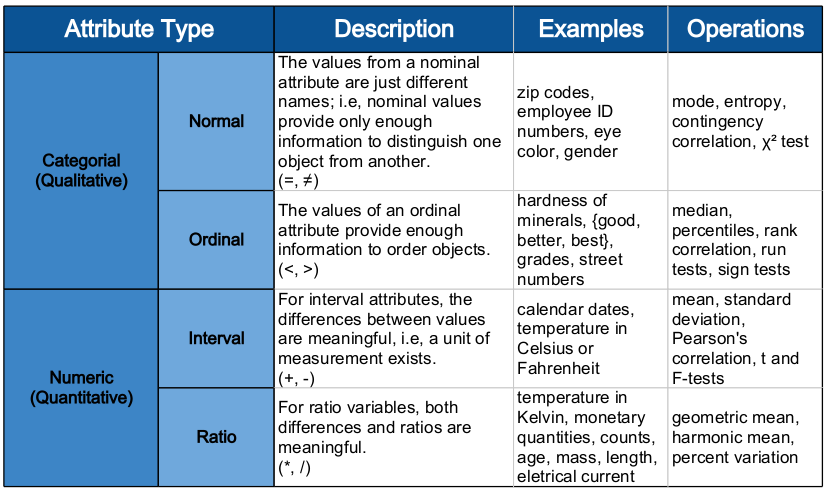
\includegraphics[width=\textwidth]{pics/typeOfAttributes.png}
		\end{figure}

	\clearpage
	\subsection*{Transformations}

		The types of attributes can be described in terms of transformations that
		do not change the meaning of an attribute. 

		\begin{figure}[H]
			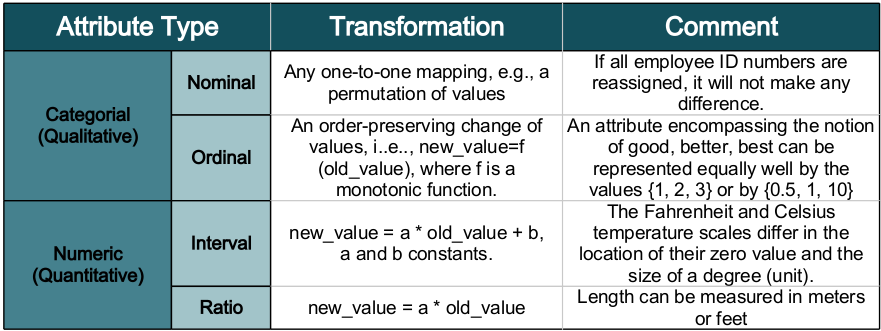
\includegraphics[width=\textwidth]{pics/transformations.png}
		\end{figure}

	\subsection*{Attributes by the Number of Values}

	An independent way of distinguishing between attributes is by the number of values
	they can take.

	\begin{itemize}
		\item {\bf Discrete:} A discrete attribute has a finite or countably infinite
		set of values. {\bf Binary attributes} are a special case of discrete attributes. 
		\item {\bf Continnuous:} A continuous attribute is one whose values are real numbers.
		\item {\bf Asymmetric:} For asymmetric attributes, only presence - a non-zero attribute
		value - is regarded as important. Binary attributes where only non-zero values are 
		important are called asymmetric binary attibutes. We can take a look at a list of all 
		courses at NTNU. If we look at a particular student, the chance for a particular student
		have taken a exam in a course from the whole list is quite small. It is only the non-zero
		values that are important. 
	\end{itemize}

	\clearpage
	\section{Type of Data Sets}

		\subsection*{General Characteristics of Data Sets}
			\begin{itemize}
				\item {\bf Dimensionality:} is the number of attributes that the object in the 
				class set possess.
				\item {\bf Sparsity:} for some data sets, such as asymmetric features, most
				attributes of an object have values of 0. In practical terms, sparsity is an advantage
				because usually only the non-zero values need to be stored an manipulated. 
				\item {\bf Resolution:} it is frequently possible to obtain data at different levels of
				resolution, and often the properties of the data are different at different resoultions.
				F.eks the surface of the Earth seems very uneven at a resolution of a few meters, but is *
				relatively smooth at a resolution of ten kilometers. The patterns in the data also depend
				on the level of resolution. Too fine will might hide the pattern or be buried in noise if
				to uneven. 
			\end{itemize}


		\clearpage
		\subsection*{Record Data}
		Much data mining work assumes that the data set is a collection of records (data objects), each of which consists of a fixed set of data fields (attributes).
			\begin{itemize}
				\item {\bf Transactions or Market Basket Data:} transaction data is a sepecial type of record
				data, where each record (transaction) involves a set of items. Transaction data is a collection
				of sets of items. 
				\item {\bf The Data Matrix:} if the data objects in a collection of data all have the
				same fixed set of numeric attributes, then the data objects can be thought of as points
				(vectors) in a multidimensional space, where each dimension represents a distinct attribute
				describing the object. 
				\item {\bf The Sparse Data Matrix:} A sparse data matrix is a special case of a data matrix in
				which the attributes are some of the same type and are symmetric; i.e, only non-zero values
				are important. {\bf Document-term matrix } is one type. 
			\end{itemize}

		\begin{figure}[H]
			\centering
			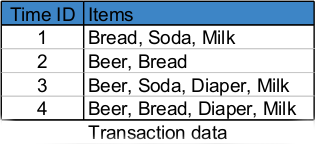
\includegraphics[scale=0.5]{pics/transactionData.png}
		\end{figure}

		\begin{figure}[H]
			\centering
			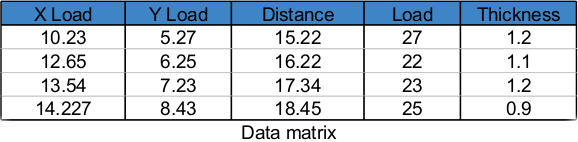
\includegraphics[scale=0.5]{pics/dataMatrix.png}
		\end{figure}

		\begin{figure}[H]
			\centering
			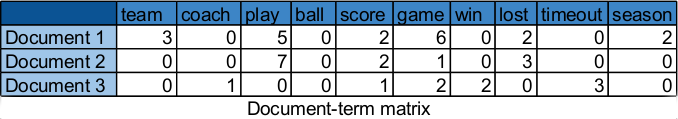
\includegraphics[scale=0.5]{pics/DocumentTermMatrix.png}
		\end{figure}

		\subsection*{Graph-Based Data}
			\begin{itemize}
				\item {\bf Data with Relationships among Objects:} the relationships among objects frequently convey important information. In such cases, the data is often represented as a graph. In 
				particular, the data objects are mapped to nodes of the graph, while the relationships among
				objects are captured by the links between objects and link propeties. 
				\item {\bf Data with Objects Thar Are Graphs:} if objects have structure, that is, the objects
				contain subobjects that have relationships, then such objects are frequently represented as graphs.
			\end{itemize}

		\clearpage
		\subsection*{Ordered Data}
		For some types of data, the attributes have relationships that involve order in time or space. 
			\begin{itemize}
				\item {\bf Sequential Data (temporal data):} can be thought of as an extension of record data, 
				where each record ha a time associated with it. 
				\item {\bf Sequence Data:} consists of a data set that is a sequence of individual entities, 
				such as a sequence of words or letters. 
				\item {\bf Time Series Data:} is a special type of sequential data in which each record is a
				time series, i.e, a series of measurements taken over time. 
				\item {\bf Spatial Data:} some objects have spatial attributes, such as positions or areas, as
				well as other type of attributes. 
			\end{itemize}

		\begin{figure}[H]
			\centering
			\subfigure{
				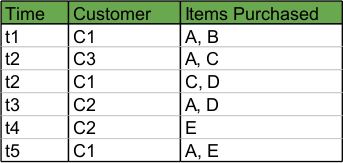
\includegraphics[scale=0.5]{pics/transactionData1.png}
			}
			\subfigure{
				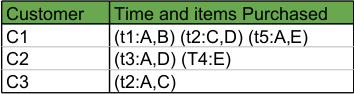
\includegraphics[scale=0.5]{pics/transactionData2.png}
			}
			\caption{Sequential transaction data}
		\end{figure}

		\begin{figure}[H]
			\centering
			\subfigure{
				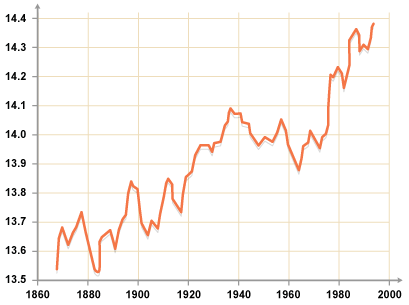
\includegraphics[scale=0.4]{pics/timeSeries.png}
			}
			\subfigure{
				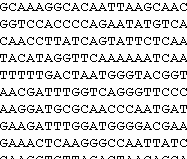
\includegraphics[scale=0.7]{pics/GenomicSequence.png}
			}
			\caption{Temperature time series and Genomic sequence data}
		\end{figure}

		\begin{figure}[H]
			\centering
			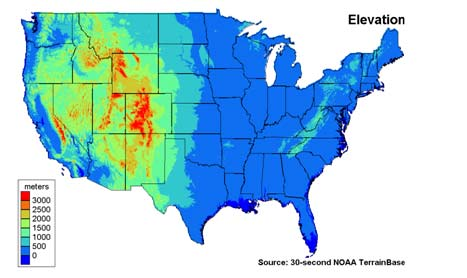
\includegraphics[scale=0.5]{pics/spatialTemp.jpg}
			\caption{Spatial temperature data}
		\end{figure}


\section{Data Quality}
	
	{\bf Data mining focuses on:}
	\begin{enumerate}
		\item The detection and correction of data quality problems (data cleaning).
		\item The use of algorithms that can tolarate poor data quality
	\end{enumerate}

	{\bf Measurement error:}
		\begin{itemize}
			\item {\bf Noise}
			\item {\bf Artifacts:} data errors may be the result of a more deterministic
			phenomenon, such as a streak in the same place on a set of photographs.
			\item {\bf Bias:} a systematic variation of measurements from the quanity
			being measured. 
			\item {\bf Precision:} the closeness of repeated measurements (of the
			same quantity) to one another.
			\item {\bf Accuracy:} the closeness of measurements to the true value
			of quantity being measured.
		\end{itemize}

	{\bf Data collection problems:}
		\begin{itemize}
			\item {\bf Outliners:} Outliners are either (1) data objects that, in some
			sense, have characteristics that are different from most of the other data
			objects in the data set, or (2) values of an attribute that are unusual with
			respect to the typical values for that attribute. It is important to distinguish
			between the notions of noise and outliners. Outliners can be legitimate data
			objects or values, unlike noise, outliners may sometimes be of interest. 
			\item {\bf Missing values:} it is not unusual for an object to be missing one 
			or more attribute values. Here are some strategies for dealing with missing values:
				\begin{itemize}
					\item Eliminate data object or attributes
					\item Estimate missing values
					\item Ingnore the missing value during analysis
				\end{itemize}
			\item {\bf Inconsistent values:} it often detected inconsistent data with manual
			typing or handwriting. It is important to correct the data as soon as possible.
			\item {\bf Duplicate data:} Often detected when there exists two objects that 
			acyually represent a single object. 
		\end{itemize}

	{\bf Issues Related to Applications}
		\begin{itemize}
			\item {\bf Timeliness:} some data starts to age as soon as it had been 
			collected. If the data is out of date, then so are the models and patterns
			that are based on it. 
			\item {\bf Relevance:} the available data must contain the information necessary
			for the application. Lack of information could give a wrong impression or patterns.
			\item {\bf Knowledge about the data:} important characteristics like precision of the
			data, the type of features (nominal, ordinal, interval, ratio), the scale of 
			measurement (e.g., meters or feet for length), and the origin of the data.
		\end{itemize}

		\vspace{1cm}

		{\LARGE "...data is of high quality if it is suitable for its intended use"}



\section{Data Preprocessing}
	
	\subsection*{Aggregation}
		\begin{itemize}
			\item Sometimes {\bf "less is more"} and this is the case with aggregation, 
			the combining of two or more objects into a single object. 
			\item {\bf Motivations for aggregation:}
				\begin{enumerate}
					\item The smaller the data sets resulting from data reduction
					require {\bf less memory and processing time}.
					\item aggregation may permit the use of {\bf expensive data mining 
					algorithms}
					\item Aggregation can act as a change of scope or scale by providing a
					high-level view of the data instead of a low-level view. 
					\item The behaviour of groups of objects or attributes is often {\bf more
					stable} than that of individual objects or attributes. 
				\end{enumerate}
			\item A {\bf disadvantage} of aggregation is the potential loss of interesting details. 
			An a store example aggregating over monthhs loses information about which day of the
			week has the highest sales. 
		\end{itemize}

	\subsection*{Sampling}
		\begin{itemize}
			\item {\bf Sampling} is a commonly used approach for selecting a subset of the data 
			objects to be analyzed. To analyze a full data set if often too expensive or 
			time consuming. 
			\item The key principle for effective sampling is the following: Using a sample
			will work almost as well as using the entire data set if the sample is 
			representative.
			\item {\bf A sample is representative if} it has approximately the same property 
			(of interest) as the original set of data. If the mean (average) of the data
			objects is the property of interest, then a sample is representative if it has
			a mean that is close to that of the original data. 
			\item {\bf Sampling approaches:}
				\begin{itemize}
					\item {\bf Simple random sampling: } for this type of sampling there is 
					an equal probability of selecting any particular item. There are two 
					variations on random sampling
						\begin{enumerate}
							\item {\bf Sampling without replacement:} as each item is selected, it is
							removed from the set of all objects that together constitute the
							population. 
							\item {\bf Sampling with replacement:} objects are not removed from 
							the population as they are selected for the sample. 
						\end{enumerate}
					{\bf Pros and cons with random sampling:}  
					(1) Sampling with replacement are is simpler to analyze since the probability 
					of selecting any object remains constant during the sampling process. 
					(2) When the population consists of different types of objects, with widely
					different numbers of objects, simple random sampling can fail to adequately
					represent those types of objects that are less frequent. This can cause
					problems when the analysis require proper representation of all object types.
					\item {\bf Stratified sampling:} starts with prespecified groups of objects.
						\begin{enumerate}
							\item In the simplest version, equal numbers of objects are drawn from 
							each group even though the groups are of different sizes. 
							\item In an other variation, the number of objects drawn from each group 
							is proportional to the size of that group. 
						\end{enumerate} 
					\item {\bf Adaptive and progressive sampling:} The proper sampling size
					can sometimes be difficult to determine. These approaches starts with a 
					small sample, and then increase the sample size until a sample of sufficient
					size has been obtained. While this technique eliminates the need to determine
					the correct sample size initially, it requires that there be a way to evaluate
					the sample to judge if it is large enough.
				\end{itemize}			
		\end{itemize}

	\subsection*{Dimensionality reduction}
		\begin{itemize}
			\item Example of data sets with a high dimentionality is a object with many
			attributes like a document object where each word in the document is an 
			attribute. 
			\item There is a varity of benefits to dimensionality reduction. A key benefit 
			is that many data mining algoithms work better if the dimensionality - 
			the number of attributes in the data - is lower. This is partly because 
			dimensionality reduction can eliminate irrelevant features and reduce noise and
			partly because of the curse of dimensionality.
			\item Another benefit is that a reduction of dimensionality can lead to a more
			understandable model because the model may involve fewer attributes.
			\item Dimensionality reduction may allow the data to be more easily visualzed.
			\item The amount of time and memory required by the data mining algorithm is reduced 
			with a reduction in dimensionality. 
			\item The term dimensionality reduction is often reserved for those techniques
			that reduce the dimensionality of a data set by creating new attributes that
			are a combination of the old attributes. 
			\item {\bf The curse of dimensionality:} the curse of dimensionality refers
			to the phenomen that many types of data analysis become significantly harder
			as the dimensionality of the data increases. 
			\item {\bf Linear alegebra techniques for dimensionality reduction:} some
			of the most common approaches for dimensionality reduction, poarticulary for
			continous data, use techniques from linear algebra to project the data from a 
			high-dimensional space into a lower-dimensional space. 
				\begin{itemize}
					\item {\bf Principal Components Analysis (PCA):} is a linear algebra technique 
					for continuous attributes that finds new attributes (principal components)
					that (1) are linear combinations of the original attributes, 
					(2) are orthogonal to each other, and (3) capture the maximum amount of 
					variation in the data. 
					\item {\bf Singular value decomposition (SVD): } is a linear algebra
					technique that is related to PCA and is also commonly used for
					dimensionality reduction.
				\end{itemize}
		\end{itemize}

	\clearpage
	\subsection*{Feature subset selection}
		\begin{itemize}
			\item A way to reduce the dimensionality is to use only a subset of the 
			features.
			\item {\bf Redundant and irrelevant features:} redundant features duplicate much 
			or all of the information contained in one or more other attributes. Irrelevant
			features contain almost no useful information for the data mining task at hand
			(feks ID number will not be relevant if we want to predict students grade).
			\item {\bf Approaches for feature selection:}
				\begin{itemize}
					\item {\bf Embedded approaches:} feature selection occurs naturally as
					a part of the data mining algorithm.
					\item {\bf Filter approaches:} features are selected before the data
					mining algorithm is run, using some approach that is independent of the
					data mining task. 
					\item {\bf Wrapper approaches:} these methods use the target data mining
					algorithm as a black box to find the best subset of attributes, in a way
					similar to that of the ideal algorithm described above, but typically 
					without enumerating all possible subsets. 
				\end{itemize}
			\item{\bf An architecture for feature subset selection:} 
			a measure for evaluating a subset, a search strategy that controls the generation 
			of a new subset of features, a stopping criterion, and a validation procedure.
				\begin{figure}[H]
					\centering
					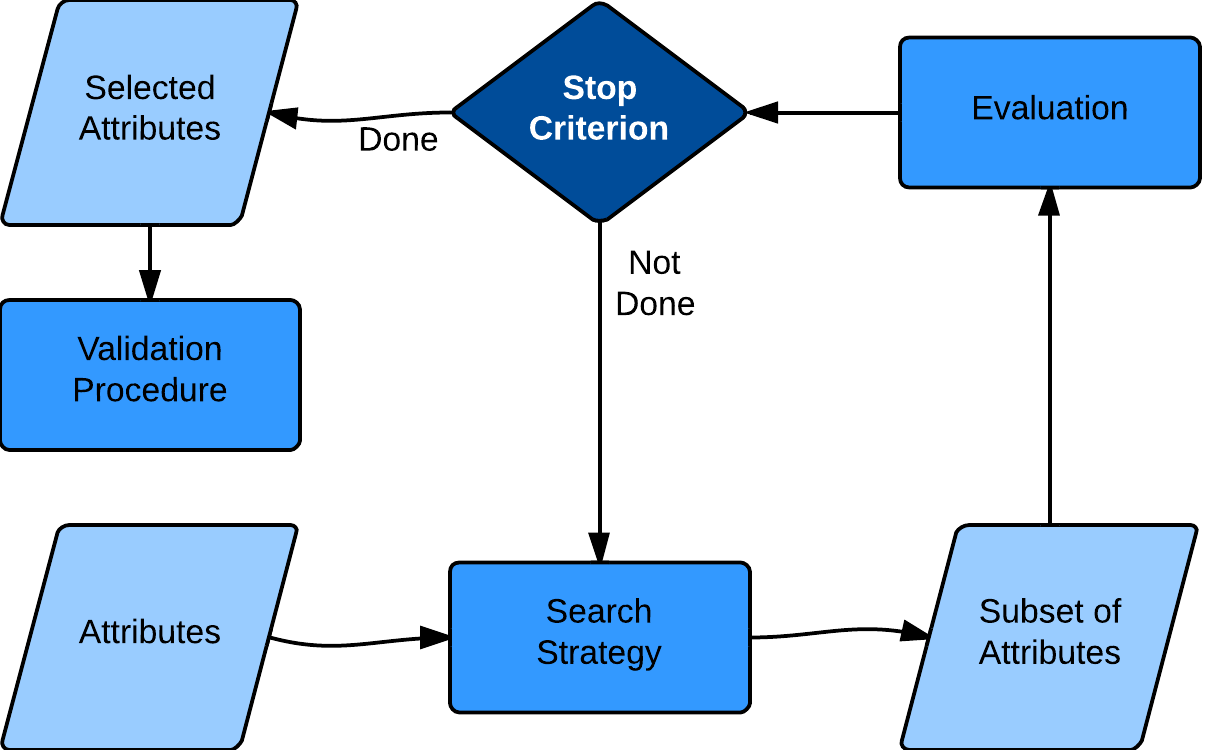
\includegraphics[scale=0.2]{pics/featureSelection.png}
				\end{figure} 
			\item{\bf Feature Wighting:} is an alternative to keeping or eliminate features.
			More important features are assigned a higher weight, while less important
			features are given a lower weight. 
		\end{itemize}

	\subsection*{Feature creation}
		\begin{itemize}
			\item It is frequently possible to create, from the original attributes, a new set
			of attributes that captures the important information in a data set much more
			effectively. 
			\item {\bf Feature extraction:} the creation of a new set of features from the 
			original raw data. 
			\item {\bf Mapping the data to a new space:} 
			\item {\bf Feature Construction: } sometimes the features in the original data sets have
			the necssary information, but is not in a form suitable for the data mining algorithm.
			In this situation, one or more new features constructed out of the original features can
			can be more useful than the original features. 
		\end{itemize}

	\subsection*{Discretization and binarization}
		\begin{itemize}
			\item Some data mining algorithms, especially certain classification algorithms, 
			require that the data be in the form of categorical attributes. 
			\item {\bf Discretization:} It is often necessary to transform a continuous attribute into a categorical attribute.
			\item {\bf Binarizaation:} both continuous and discrete attributes may need to be 
			transformed into one or more binary attributes.
			\item If a categorical attribute has a large numer of values (categories), or some
			values occur infrequently, then it may be beneficial for certain data mining tasks
			to reduce the number of categories by combining some of the values. 
		\end{itemize}

	\subsection*{Variable transformation}
		\begin{itemize}
			\item A {\bf variable transformation} refers to a transformation that is applied to
			all the values of a variable. 
			\item{\bf Types of variable transformations:}
				\begin{itemize}
					\item{\bf Simple functions:} for this type of variable transformation, a 
					simple mathematical function is applied to each value individually. 
					\item{\bf Normalization and standardization:} the goal of standardization 
					or normalization is to make an entire set of values have a particular 
					property. 
				\end{itemize}
		\end{itemize}

\clearpage
\section{Measures of Similarity and Dissimilarity}

	\begin{itemize}
		\item {\bf Proximity:} the term is used to refer to either similarity or dissimilarity
		\item {\bf Similarity:} similarity between two objects is a numerical measure of the degree 
		to which the two objects are alike.
		\item{\bf Dissimilarity:} dissimilarity between two objects is a numerical measure of the 
		degree to which the two objects are different.
		\item {\bf Transformations:} are often applied to convert a similarity to a dissimilarity
		or vice versa, or to transform a proximity measure to fall within a particular range,
		such as [0, 1].
	\end{itemize}

	\subsection*{Similarity and Dissimilarity between Simple Attributes}

		\begin{itemize}
			\item{\bf Nominal:} since nominal attributes only convey information about
			the distinctness of objects, all we can say is that two objects either have the
			same value or they do not.
			\item{\bf Ordinal:} for objects with a single ordinal attribute, the situation
			is more complicated because information about order should be taken into account.
			Consider an attribute that measures the quality of a product, e.g., a candy bar, 
			on the scale {poor, fair, OK, good, wonderful} = {poor=0, fair=1, OK=2, good=3, 
			wonderful=4}.
			\item{\bf Ratio:} for interval or ratio attributes, the natural measure of dissimilarity
			between two objects is the absolute difference of their values.
		\end{itemize}

		\begin{figure}[H]
			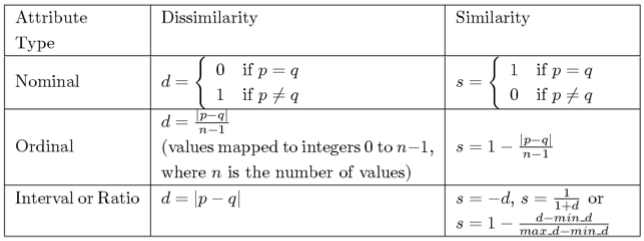
\includegraphics[width=\textwidth]{pics/simpleAttribute.png}
		\end{figure}

	
	\subsection*{Dissimilarities between Data Objects}

	{\bf Euclidean distance:} The euclidean distance, d, between two points, x and y,
	in one-, two-, three-, or higher dimensional space, is given by the following formula:

		$d(x,y) = \sqrt{\sum_{k=1}^{n} (x_k - y_k)^{2}}$
	

	where n is the number of dimensions, and xk and yk are repsectively the k'th attibutes
	of x and y. 

	\clearpage
	{\bf Minkowski distances:}


		$d(x,y) = \left(\sum_{k=1}^{n} |x_k - y_k|^{r}\right) ^{1/r}$

	\begin{itemize}
		\item {\bf r = 1} City block (Manhattan, txicab, $L_{1}$ norm) distance.
		\item {\bf r = 2} Euclidean distance ($L_{2}$ norm).
		\item {\bf r = $\infty$} Supremum ($L_{max}$ or $L_{\infty}$) distance.
	\end{itemize}

	Distances, such as the Eucledian distance, have some well-known properties. if
	d(x,y) is the distance between two points, x and y, then the following properties
	hold:

		\begin{enumerate}
			\item {\bf Positivity}
			\begin{enumerate}
				\item d(x,y) $\geq$ for all x and y,
				\item d(x,y) = 0 only if x = y
			\end{enumerate}
			\item {\bf Symmetry} \\
				d(x,y) = d(y,x) for all x and y
			\item {\bf Triangle Inequality} \\
				d(x,z) $\leq$ d(x,y) + d(y,z) for all points x, y, and z
		\end{enumerate}

	{\bf Metrics: } measures that satisfy all three properties are known as metrics.

	\begin{table}[H]
		\centering
		\begin{tabular}{| l | l | l |}
			\hline
			point & x coordinate & y coordinate \\ \hline
			p1 & 0 & 2 \\ \hline
			p2 & 2 & 0 \\ \hline
			p3 & 3 & 1 \\ \hline
			p4 & 5 & 1 \\ \hline
		\end{tabular}
		\begin{tabular}{| l | l | l | l | l |}
			\hline
			 & p1 & p2 & p3 & p4 \\ \hline
			p1 & 0.0 & 2.8 & 3.2 & 5.1 \\ \hline
			p2 & 2.8 & 0.0 & 1.4 & 3.2 \\ \hline
			p3 & 3.2 & 1.4 & 0.0 & 2.0 \\ \hline
			p4 & 5.1 & 3.2 & 2.0 & 0.0 \\ \hline
		\end{tabular}
		\caption{(a) x and y coordinates, (b) Euclidean distance matrix}
	\end{table}

	\begin{table}[H]
		\centering
		\begin{tabular}{| l | l | l | l | l |}
			\hline
			$L_{1}$ & p1 & p2 & p3 & p4 \\ \hline
			p1 & 0.0 & 4.0 & 4.0 & 6.0 \\ \hline
			p2 & 4.0 & 0.0 & 2.0 & 4.0 \\ \hline
			p3 & 4.0 & 2.0 & 0.0 & 2.0 \\ \hline
			p4 & 6.0 & 4.0 & 2.0 & 0.0 \\ \hline
		\end{tabular}
		\begin{tabular}{| l | l | l | l | l |}
			\hline
			$L_\infty$ & p1 & p2 & p3 & p4 \\ \hline 
			p1 & 0.0 & 2.0 & 3.0 & 5.0 \\ \hline
			p2 & 2.0 & 0.0 & 1.0 & 3.0 \\ \hline
			p3 & 3.0 & 1.0 & 0.0 & 2.0 \\ \hline
			p4 & 5.0 & 3.0 & 2.0 & 0.0 \\ \hline
		\end{tabular}
		\caption{(a) $L_{1}$ distance matrix, (b) $L_{\infty}$ distance matrix}
	\end{table}

\subsection*{Similarities between Data Objects}
	If s(x,y) is the similarity between points x and y, then the typical properties
	of similarities are the following:
		\begin{enumerate}
			\item s(x,y) = 1 only if x = y. (0 $\leq$ s $\geq$ 1)
			\item s(x,y) = s(y,x) for all x anf y. (Symmetry)
		\end{enumerate}

\subsection*{Examples}

	{\bf Similarity Measures of Binary Data:}

	Similarity measures between objects that contain only binary attributes are called
	similarity coefficients, and typically have values between 0 and 1.
	Let x and y be two objects that consist of n binary attributes. The comparison 
	of two such objects, i.e., two binary vectors, leads to the following four quantities
	(frequancies):

		$f_{00}$ = the number of attributes where x is 0 and y is 0 \\
		$f_{01}$ = the number of attributes where x is 0 and y is 1 \\
		$f_{10}$ = the number of attributes where x is 1 and y is 0 \\
		$f_{11}$ = the number of attributes where x is 1 and y is 1 \\

	{\bf Simple Matching Coefficient (SMC)} one commonly used similarity coefficient, 
	which is defined as: \\

		SMC = $\frac{number of matching attribute values}{number of attributes}$ = 
		$\frac{f_{11} + f_{00}}{f_{01} + f_{10} + f_{11} + f_{00}}$
		\\


	{\bf Jaccard Coefficient} is frequently used to handle objects consisting of 
	asymmetric binary attributes. The Jaccard coefficient, which is often symolized by J, 
	is given by the following equation: \\

		$J = \frac{number of matching presences}{number of attibutes not involved in 00 matches} =
		\frac{f_{11}}{f_{01} + f_{10} + f_{11}}$
		\\

	{\bf Cosine Similarity} \\ 

		cos(x,y) = $\frac{x*y}{\|x\| \|y\|}$
		\\

	{\bf Extended Jaccard Coefficient} \\

		EJ(x,y) = $\frac{x*y}{\|x\|^{2} + \|y\|^{2} - x*y}$
		\\

	{\bf Correlation} between two data objects that have binary or continuous variables is a
	measure of the linear relationship between the attributes of the objects. 
	{\bf Pearson's correlation} coefficient between two data objects, x and y, is defined
	by the following equation: \\

		corr(x,y) = $\frac{covariance(x,y)}{standardDeviation(x)*standardDeviation(Y)}$ = 
		$\frac{s_{xy}}{s_{x}s_{y}}$


	


